\newpage
\section{Durchführung}
\subsection{Aufgabenteil a)}
Zur Bestimmung der Dämpfungskonstante einer gedämpften harmonischen Schwingung wird der Versuch nach Abbildung (\ref{fig:aufbaua}) aufgebaut.

\begin{figure}
    \centering
       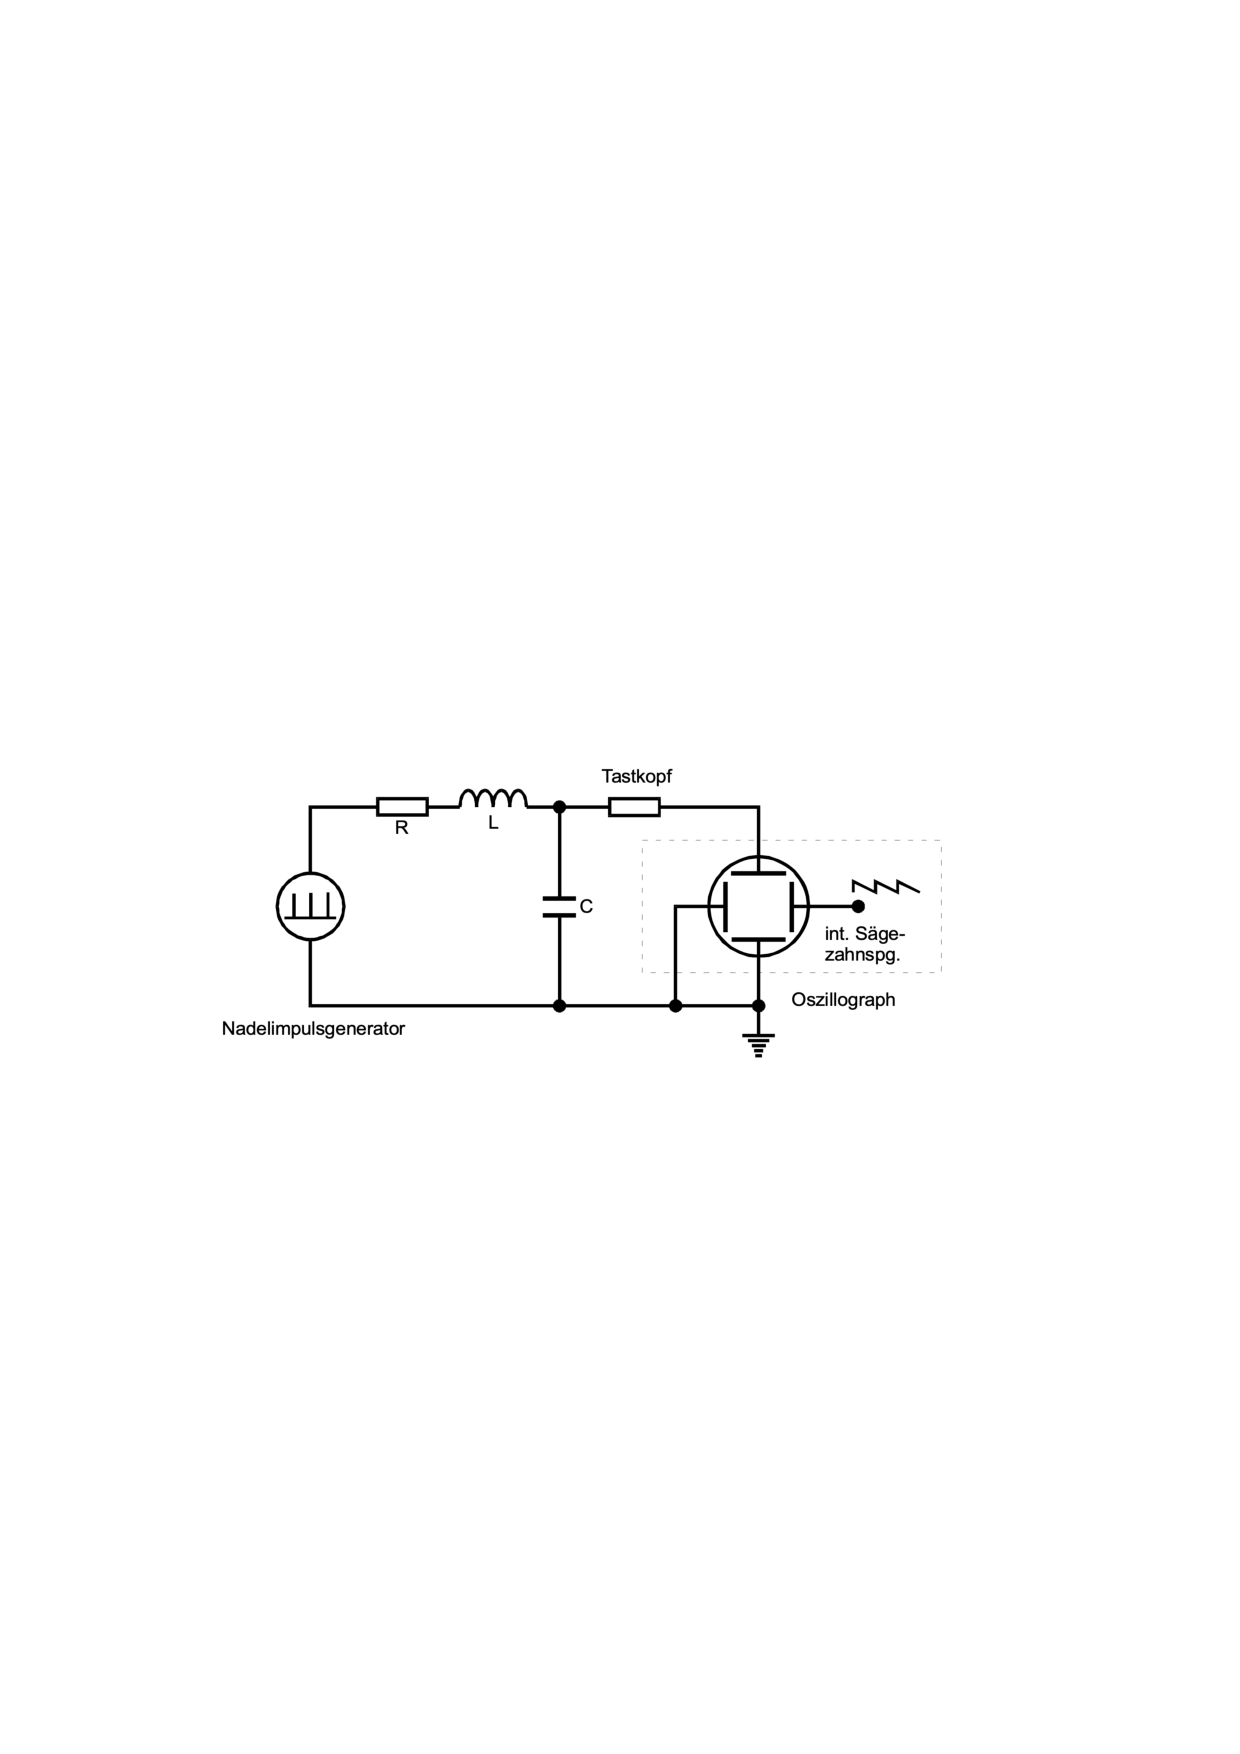
\includegraphics[height=5cm]{aufbaua.pdf}
       \caption{Aufbau zur Untersuchung der Zeitabhängigkeit der Amplitude einer gedämpften Schwingung (Quelle: \cite{V354}).}
       \label{fig:aufbaua}
\end{figure}

\noindent
Dann werden möglichst viele Amplituden auf dem Oszillographen vermessen sowie die dazugehörigen Zeiten aufgenommen und notiert.
Die Ergebnisse befinden sich in Tabelle (\ref{tab:1}).

\subsection{Aufgabenteil b)}
Um den Dämpfungswiderstand $R_{ap}$ zu bestimmen, 
bei dem der aperiodische Grenzfall eintritt,
wird der Versuch nach Abbildung (\ref{fig:aufbaub}) aufgebaut.

\begin{figure}
    \centering
       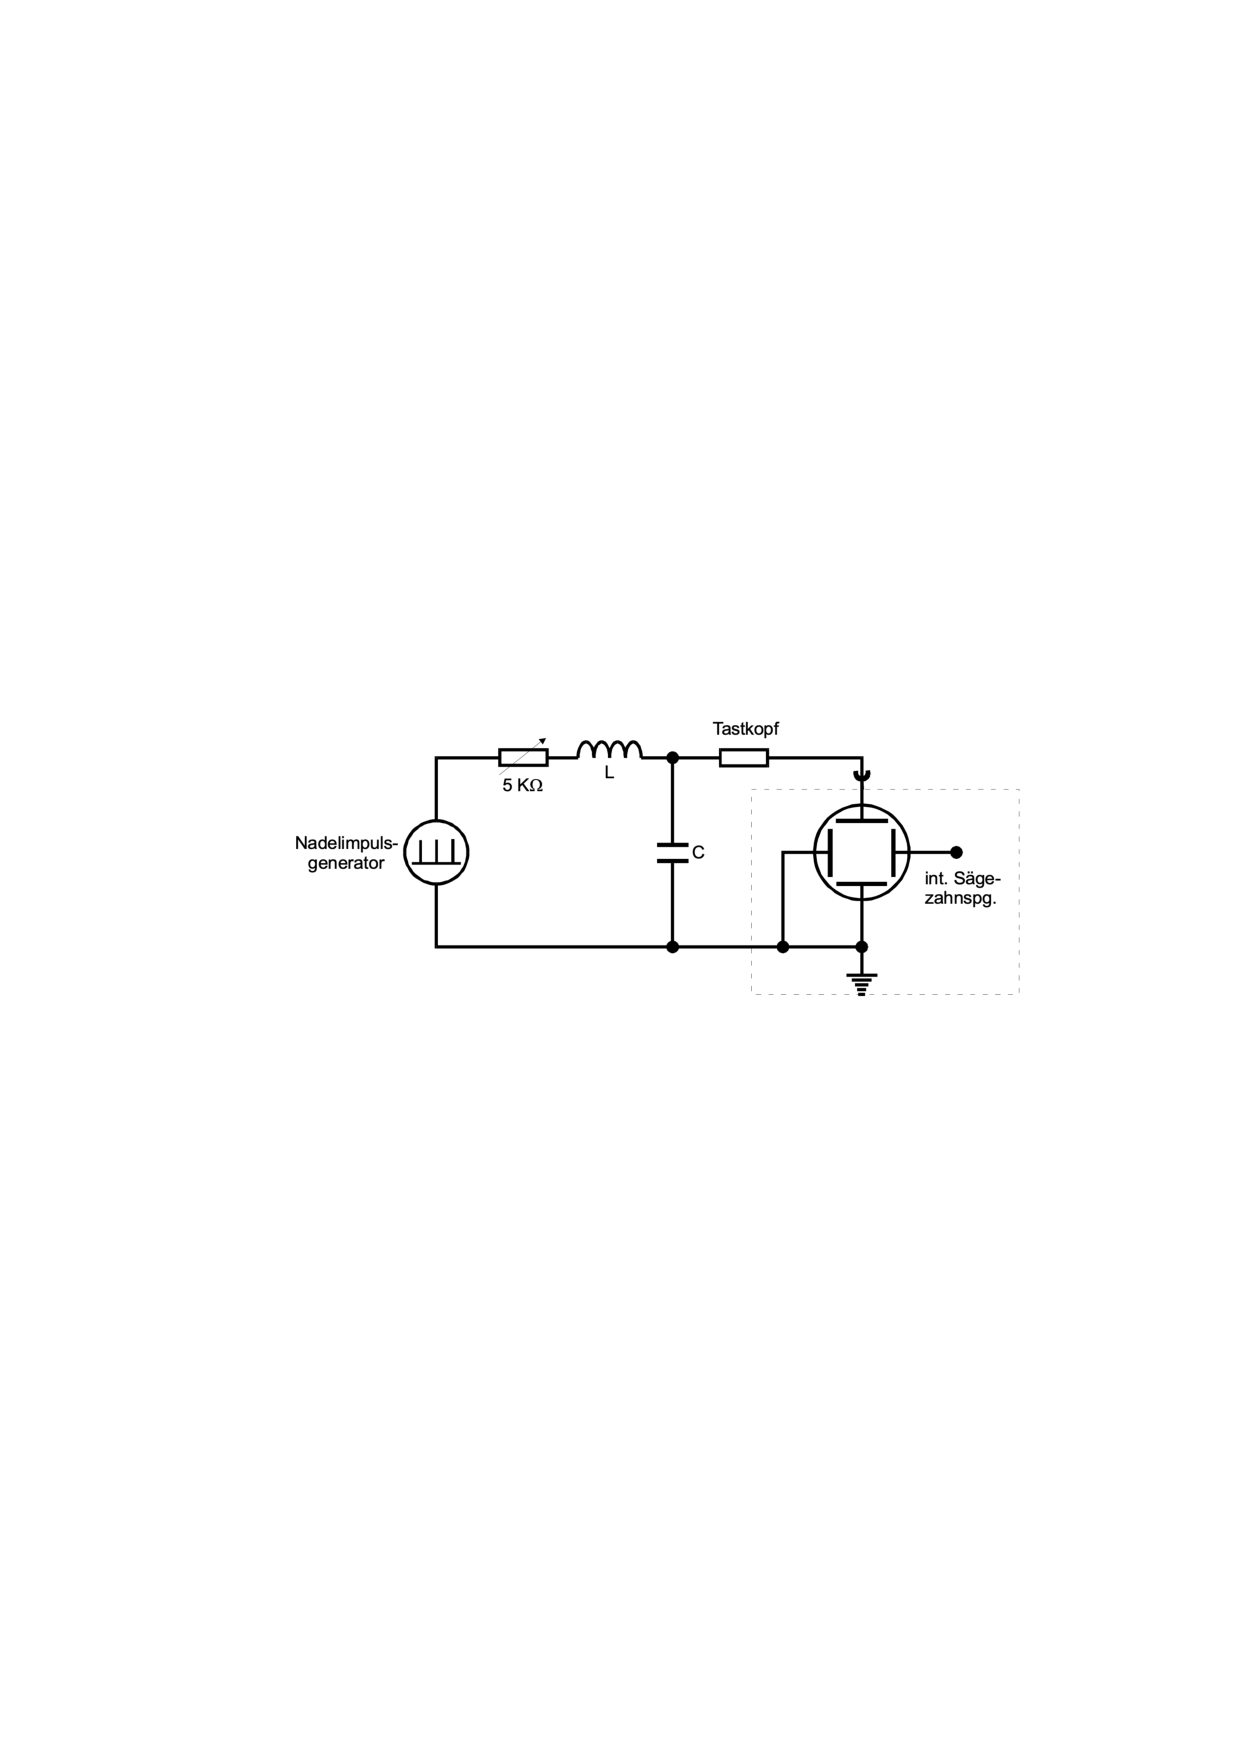
\includegraphics[height=5cm]{aufbaub.pdf}
       \caption{Aufbau zur Untersuchung des Widerstandes für den aperiodischen Grenzfall (Quelle: \cite{V354}).}
       \label{fig:aufbaub}
\end{figure}

\noindent
Nun wird der regelbare Widerstand so lange variiert,
bis die Kondensatorspannung die auf dem Oszillographen beobachtet wird,
ohne Überschwingen am schnellsten gegen Null geht 
(analog zur gestrichelten Linie aus Abbildung (\ref{fig:grenzfall})).
Der Wert des Widerstandes wird von der Skala abgelesen wird notiert.

\subsection{Aufgabenteil c)}
Um die Frequenzabhängigkeit der Kondensatorspannung zu untersuchen, 
wird der Versuch nach Abbildung (\ref{fig:aufbauc}) aufgebaut.

\begin{figure}
    \centering
       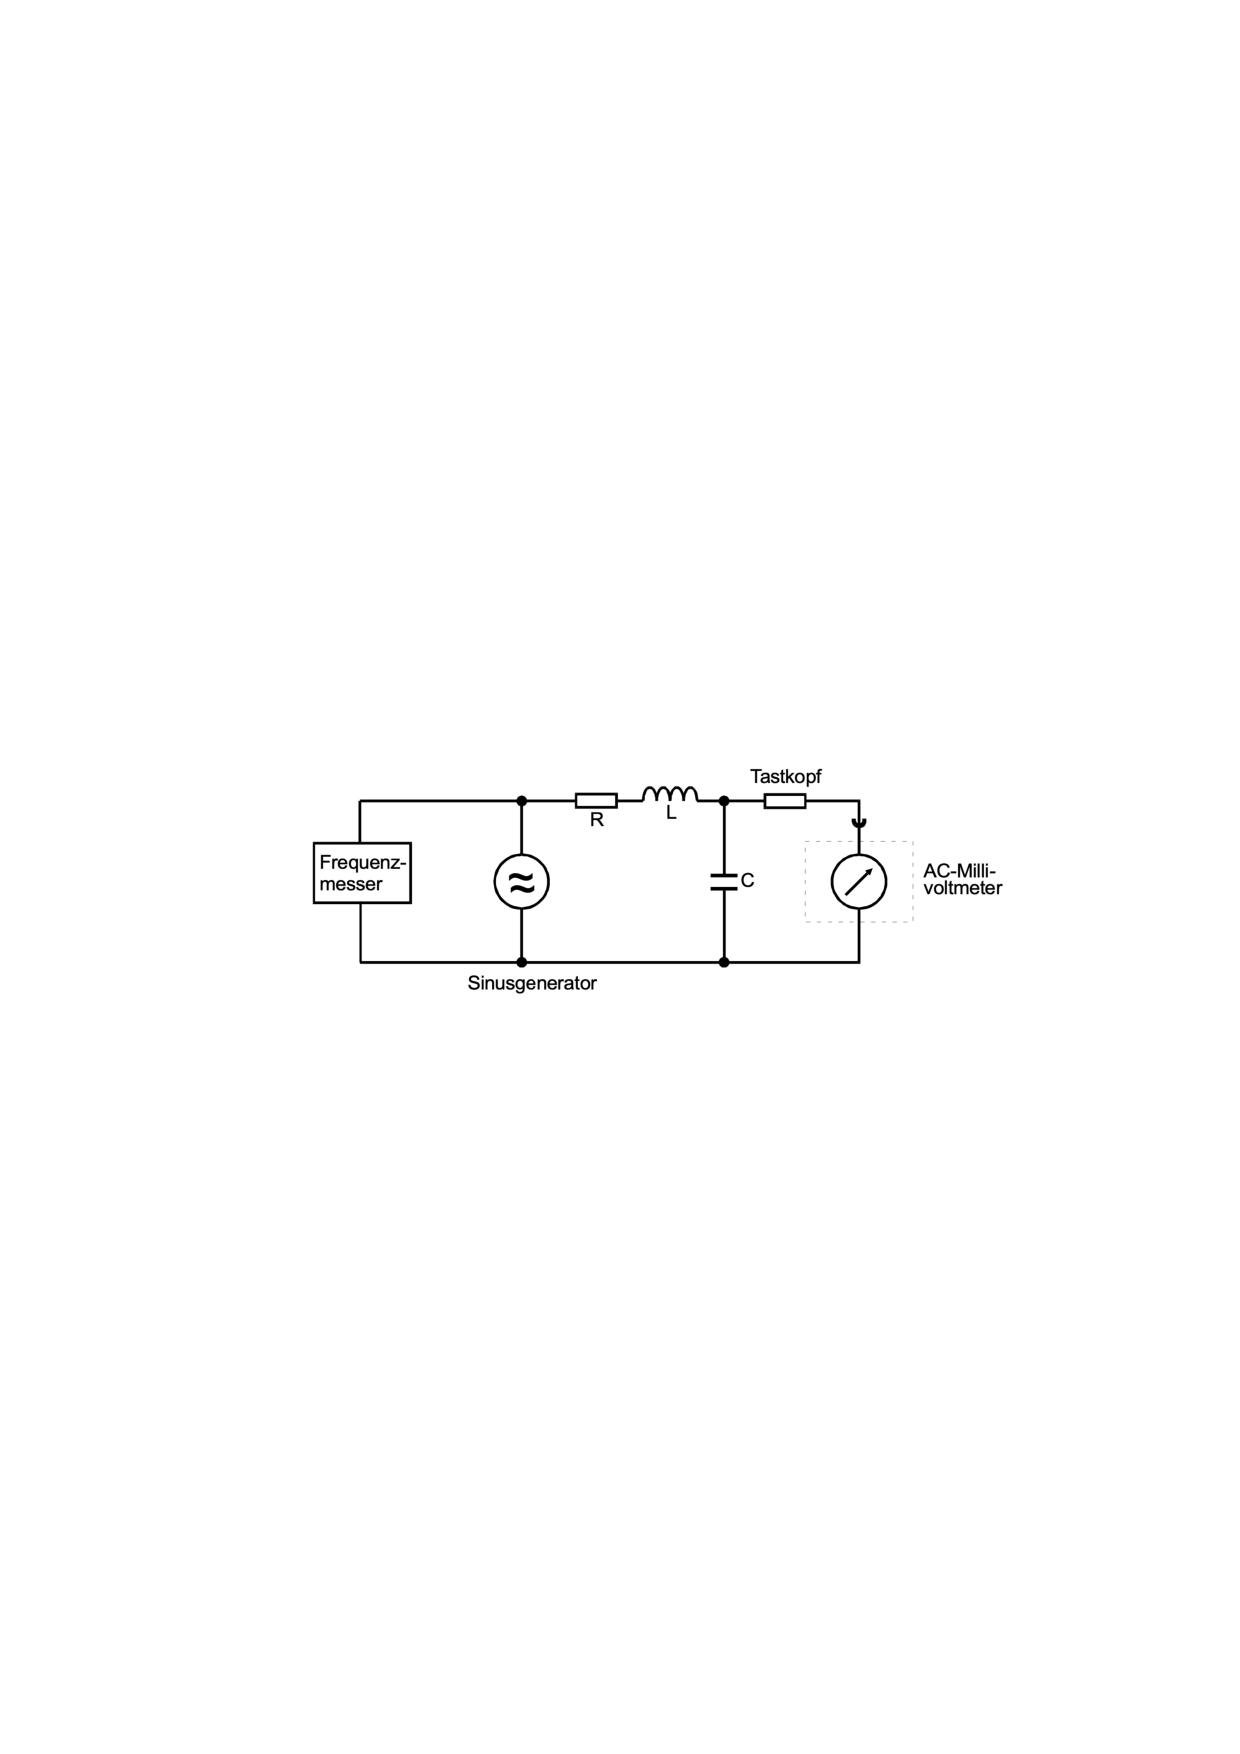
\includegraphics[height=5cm]{aufbauc.pdf}
       \caption{Aufbau zur Aufnahme des Frequenzganges eines RLC-Kreises (Quelle: \cite{V354}).}
       \label{fig:aufbauc}
\end{figure}

\noindent
Anschließend wird die Frequenz von 5kHz bis 60kHz in regelmäßigen Abständen erhöht, 
wobei im Bereich um die Resonanzfrequenz mehr Messdaten aufgenommen werden.
Zu jeder eingestellten Frequenz wird die Kondensatorspannung $U_C$ sowie die Erregerspannung $U$ mithilfe des Oszillographen vermessen
und notiert.
Die Messdaten hierzu befinden sich in Tabelle %(\ref{tab:2}).

